\documentclass[11pt,a4paper,openany]{book}

%\usepackage[german]{babel}	%in case you want to write a german thesis

%settings for generation of titlepage, index and table of content
\usepackage{graphicx}
\usepackage{geometry}
\usepackage{fancyhdr}
\usepackage{tabularx}
\usepackage[
indexing=cite,
backend=biber,
sorting=nyt,
maxcitenames=1, 
mincitenames=1, 
maxbibnames=999, 
minbibnames=999,
refsection=section,
autocite=footnote,
doi=true,
url=true,
style=authortitle-ibid
]{biblatex}
\usepackage{makecell}
\usepackage{titlesec}
\usepackage{lipsum}
\usepackage[super]{nth}
\usepackage{imakeidx}
\usepackage{hyperref}
\usepackage{listings}
\usepackage{color}
\usepackage{footnote}
\usepackage{amsmath}


\definecolor{dkgreen}{rgb}{0,0.6,0}
\definecolor{gray}{rgb}{0.5,0.5,0.5}
\definecolor{mauve}{rgb}{0.58,0,0.82}
\definecolor{orange}{RGB}{255,143,0}
\definecolor{dkblue}{rgb}{0.14, 0.13, 0.35}
\definecolor{brown}{rgb}{0.321, 0.105, 0.113}

\lstset{frame=tb,
	language=python,
	aboveskip=5mm,
	belowskip=5mm,
	showstringspaces=false,
	columns=flexible,
	basicstyle={\small\ttfamily},
	numbers=left,
	numberstyle=\tiny\color{gray},
	keywordstyle=\color{orange},
	commentstyle=\color{dkgreen},
	stringstyle=\color{mauve},
	breaklines=true,
	breakatwhitespace=false,
	tabsize=4
}

\pagestyle{fancy}
\fancyhf{}
\setlength{\headheight}{45pt}

\lhead{
  
\includegraphics[width=3cm]{img/htlwrn_logo}  
}
\chead{\Large HTBLuVA Wiener Neustadt \\ \normalsize Höhere Lehranstalt für Informatik}
\rhead{
  
\includegraphics[width=3cm]{img/htlwrn_logo2}
}

\newcommand{\parseauthor}[3]{\makecell{#1 \\ #2} & & #3}

\def \title {\Huge \bf D\,I\,P\,L\,O\,M\,A\,R\,B\,E\,I\,T}

\setlength{\parindent}{0em}

\geometry{
 a4paper,
 left=30mm,
 top=50mm,
 }
 
\graphicspath{ {img/} }

\makeindex[title=Index]
\makeindex[name=allgemein, title=Common Index]
\makeindex[name=name,title={Authors Index}]
	% do not even think about changing this from name to author
\makeindex[name=title,columns=1,title={Literature Index}]
\indexsetup{level=\subsection*, toclevel=subsection, noclearpage}


\makeatletter
\@ifpackageloaded{biblatex_legacy}
{\DeclareIndexNameFormat{default}{%
		\usebibmacro{index:name}{\index[name]}{#1}{#3}{#5}{#7}}}
{\DeclareIndexNameFormat{default}{%
		\usebibmacro{index:name}{\index[name]}
		{\namepartfamily}
		{\namepartgiven}
		{\namepartprefix}
		{\namepartsuffix}}}
\makeatother

\DeclareIndexFieldFormat{indextitle}{%
	\usebibmacro{index:title}{\index[title]}{#1}}

\renewbibmacro*{bibindex}{%
	\ifbibindex
	{\indexnames{author}%
		\indexnames{editor}%
		\indexnames{translator}%
		\indexnames{commentator}%
		\indexfield{indextitle}}
	{}}

\makeatletter
\DeclareCiteCommand{\repeatfootcite}[\cbx@wrap]
{\gdef\cbx@keys{}}
{\xappto\cbx@keys{\thefield{entrykey},}}
{}
{\ifcsundef{cbx@lastin@\cbx@keys @\strfield{postnote}}
	{\csnumgdef{cbx@lastin@\cbx@keys @\strfield{postnote}}{-1}}{}%
	\ifsamepage{\value{instcount}}{\csuse{cbx@lastin@\cbx@keys @\strfield{postnote}}}
	{\footnotemark[\csuse{cbx@lastfn@\cbx@keys @\strfield{postnote}}]}
	{\xappto\cbx@cite{\noexpand\footcite%
			[\thefield{prenote}][\thefield{postnote}]{\cbx@keys}%
			\csnumgdef{cbx@lastfn@\cbx@keys @\strfield{postnote}}{\value{\@mpfn}}%
			\csnumgdef{cbx@lastin@\cbx@keys @\strfield{postnote}}{\value{instcount}}}}}

\newrobustcmd{\cbx@wrap}[1]{#1\cbx@cite\gdef\cbx@cite{}}
\def\cbx@cite{}
\makeatother

%Messbox zur Druckkontrolle:
\newcommand{\Messbox}[2]{% Parameters: #1=Breite, #2=Hoehe
	\setlength{\unitlength}{1.0mm}%
	\begin{picture}(#1,#2)%
	\linethickness{0.05mm}%
	\put(0,0){\dashbox{0.2}(#1,#2)%
		{\parbox{#1mm}{%
				\centering\footnotesize 
				%{\bf MESSBOX}\\ 
				Breite $ = #1 {\rm\ mm}$\\
				H\"ohe $ = #2 {\rm\ mm}$
	}}}\end{picture}
}

%change hyperref colors
\hypersetup{
	colorlinks = true,
	linkcolor = brown,
	filecolor = blue,
	citecolor = dkblue,      
	urlcolor = dkblue,
}

%suppress visited on ... in footnotes
\AtEveryCitekey{\clearfield{urlyear}}
\AtEveryCitekey{\clearfield{url}}
\AtEveryCitekey{\clearfield{year}}


%definitions for easier costumization
\def \subtitle {Autonomous universal Mapping and Navigation}
\def \year {2020/21}
\def \authors { \parseauthor{Themengebiet 1}{Lukas Leskovar}{5BHIF}\\
                \parseauthor{Themengebiet 2}{Fabian Kleinrad}{5BHIF}}
\def \supervisor {MMag. Dr. Michael Stifter}
\def \declauthors{ Lukas Leskovar & Fabian Kleinrad}	% for two authors
% \def \declauthors{ Vor- und NACHNAME & Vor- und NACHNAME \\ Vor- und NACHNAME}	% for three authors

\addbibresource{main.bib}

\begin{document}
	\pagenumbering{none}
	
	%include titlepage
	\begin{titlepage}
  \thispagestyle{fancy}
  \begin{center}
    \Huge
    \texttt{\textbf{\title}} \\
    \vspace{1cm}
    \LARGE
    \bf{\subtitle}\\
  \end{center}
  \vspace{2cm}
  \begin{flushleft}
    \normalsize
    \textbf{Ausgeführt im Schuljahr \year \ von:}\\
    \vspace{2mm}
     \begin{tabularx}{\linewidth}{lXr}
        \authors
      \end{tabularx} \\
  \end{flushleft}
  \vfill
  \begin{center}
      \vspace{1cm}
      \textbf{Betreuer / Betreuerin:}\\
    \vspace{2mm}
    \begin{tabular}{l}
      \supervisor
    \end{tabular}
    
    \vspace{2cm}
    
    Wiener Neustadt, am 4. April 2022
    
    \rule{14cm}{0.4mm}
    
    \begin{tabular}{p{.4\textwidth}p{.4\textwidth}}
      \scriptsize{Abgabevermerk:} & \scriptsize{Übernommen von:}
    \end{tabular}
    
  \end{center}
\end{titlepage}

	
	%include acknowledgements, abstract and documentation
	
	\pagestyle{plain}
	
%	\frontmatter
	
	\pagenumbering{roman}
	% english word for 'eidestattliche erklärung?'

\chapter{Eidestattliche Erklärung}

\vspace{10mm}

\normalsize
Hiermit erkläre ich an Eides statt, dass ich die vorliegende Arbeit selbstständig und ohne fremde Hilfe verfasst und keine anderen als die im Literaturverzeichnis angegeben Quellen und Hilfsmittel verwendet habe. Insbesondere versichere ich, dass ich alle wörtlichen und sinngemäßen Übernahmen aus anderen Werken als solche kenntlich gemacht habe.

\vspace{1cm}

Wiener Neustadt am 4. April 2022 \\

\vspace{1cm}

{\bf Verfasser:} \\

\renewcommand{\arraystretch}{5}
  \begin{tabular}{p{.4\textwidth}p{.4\textwidth}}
    \declauthors
  \end{tabular}
\renewcommand{\arraystretch}{1}
	
	\tableofcontents
	
	\chapter{Acknowledgement}

First and foremost, the authors would like to thank F-WuTS and robo4you for providing the equipment and facilities used during the development of the Autumn project. Furthermore, we want to thank our supervisor MMag. Dr. Michael Stifter, who's support, motivation and advice were of integral importance for the authors and this thesis.\linebreak

\textbf{Author: Fabian Kleinrad}

My gratitude is due to all the people who have helped me with topic or non-topic specific questions. This made realizing this project possible and directly affected the quality of the outcome. 
Especially I would like to express my thanks to Mag. Michael Krebs for proofreading reading our diploma thesis.

\textbf{Author: Lukas Leskovar}

%This thesis required a lot of effort and motivation. Fabian Kleinrad and his excellent work always pushed me to perform harder than I would've ever been alone. For this, I am very thankful. 

I would also like to thank everyone who read this thesis and contributed insight from a non-technical standpoint, improving its overall quality and readability. 

Most notably, I am very grateful for my family and friends and their support throughout the past five years. 

	\chapter{Kurzfassung}

\vspace{10mm}

Heutzutage unterstützen uns Computer mehr als je zuvor in allen Bereichen unserer Arbeit. Von digital gestürzter Gebäudekonstruktion, bis hin zu Computer basierter Waldwachsbeurteilung. Autumn bietet hierbei eine Lösung, diese Vorhaben durch eine autonome und universell einsetzbare Drohne zu vereinfachen. Die Drohne erstellt ein realitätsnahes 3-D Modell der Umgebung. Dies kann beispielsweise genutzt werden, um Maße zu entnehmen oder eine Momentaufnahme eines Vorhabens festzuhalten. Aufgrund der verwendeten Technologien ist die Drohne unabhängig von äußeren Lokalisierungsmechanismen und kann dadurch in abgelegenen Geländen eingesetzt werden. Realisiert wird dies durch den Einsatz eines SLAM-Algorithmus, um das Mapping zu ermöglichen, und einen RRT* Algorithmus für die Pfadfindung.

\chapter{Abstract}

\vspace{10mm}

Computers nowadays are integrated into a wide variety of processes. Ranging from computer-aided construction to software-based monitoring of forests. Autumn proposes a solution of using an autonomous and universally deployable drone to simplify these tasks. The drone generates a realistic model of the environment, which can be used to extract measurements or capture the momentary progress. Furthermore, autumn uses technologies that enable the drone to work independently of any external localisation mechanism, which allows for deployment in secluded areas. This characteristic can be realised by using a SLAM algorithm, needed to map the environment in combination with an RRT* algorithm, which handles the path-planning.

	
	%include thesis
	
	\mainmatter
	\pagenumbering{arabic}
	
	\chapter{Introduction}

\textbf{Author: Vor- und Nachname}

\vspace{2mm}

\lipsum[1-3]

\section{Section}
More text. \lipsum[1] See Figure~\ref{pic:example}.

\begin{figure}[h]
	\centering
	\includegraphics[width=2.5in]{img/example.png}
	\caption{Picture description.}
	\label{pic:example}
\end{figure}

\subsection{Subsection}
\lipsum[1]

\subsection{Subsection}
\lipsum[1] See Table~\ref{tab:example}.

\begin{center}
	\begin{tabular}{| l | l | l |}
		\hline
		\bfseries Header 1 & \bfseries Header 2 & \bfseries Header 2 \\
		\hline
		Text & text & text \\
		\hline
		Text & text & text  \\
		\hline
		Text & text & text  \\
		\hline
	\end{tabular}
	\label{tab:example}
\end{center}



\lipsum[1] Some references can be found at \footcite{robo4you} or at  \footcite{Hope_Learning_TensorFlow}. 


\filbreak

	\chapter{Study of Literature}

\textbf{Author: } 


\filbreak
	
	\chapter{Robot Operating System}
\label{chapter:ros}

\textbf{Author: Lukas Leskovar} 

This chapters objective is to describe the basic concepts of the Robot Operating System (ROS) utilized by Autumn. The ROS despite its name is a meta-operating system or middleware providing the utility and services often found in robotics frameworks. It enables the composition of distributed systems by utilizing publisher-subscriber communication between different programs of such systems. Furthermore ROS provides a comprehensive set of tools enabling the compilation, operation as well as testing, visualization and debugging of robotic systems. With its vast amount of libraries and huge open-source community providing useful functionality ROS facilitates the development of robotic applications without having to reimplement standardized technology. \footcite{openSourceRoboticsFoundationDefinitionNodate}


\section{Conceptual Overview}
The Robot Operating System can be divided into three conceptual levels each contributing a integral part to the utility of ROS. These different levels are described in the following sections. \footcite{openSourceRoboticsFoundationConceptsNodate}

\subsubsection{File System}
The File System Level mainly provides constraints and best practices for creating and structuring packages and their components. 
ROS provides appropriate tools to facilitate file-system operations with and within packages.
%operations such as searching for packages or file within packages
%With appropriate tooling the ROS facilitates file-system operations within packages, messages or topics. 

\subsubsection{Computational Graph}
The Computational Graph provides crucial functionality to ROS as it refers to the peer-to-peer mesh network of processes (nodes) each providing data to be utilized within the graph by publishing and subscribing to topics.
The concepts and technologies powering the computational graph are described in later in this chapter.

\subsubsection{Community}
The Community preserves the usability of ROS as new and useful packages and tools are created as well as existing functionality is being maintained.

\section{Naming}
To aid the organization of programs, processes as well as resources ROS provides two naming schemes that are described in the following sections. \citereset\footcite{openSourceRoboticsFoundationConceptsNodate}

\subsubsection{Graph Resource Names}
Graph Resource Names utilize a hierarchical structure to organize nodes, services, topics or anything else within the computational graph. ROS defines four different types of names:
%\begin{itemize}
%	\item base names - Are resolved in the same fashion as relative names
%	\item relative names - Are resolved relatively starting by the nodes name
%	\item global names - Begin with a / and are considered fully resolved
%	\item private names - Begin with a $\tilde{ }$ and convert the nodes name into a namespace
%\end{itemize}

\subsubsection{Package Resource Names}
Package Resource Names aim to facilitate the search process of resources at File System Level. These names usually consist of the packages name as well as the path to the desired resource within the package. 
%Examples for such Names are:
%\begin{itemize}
%	\item 
%\end{itemize}

\section{Packages}
Software in ROS is organized in packages containing nodes, libraries or any other piece of software providing functionality.

%noch ein bisschen trennen (atomic build item, ...)
%der absatz gefällt mir nicht, eigentlich gehört da nur die atomicity hin
%In order to maintain reusability, atomicity and easy decoupling of functionality packages aim to be as slim as possible by implementing only a limited-set of features. This means that each package is develop to focus on one task alone and work together with other packages to deliver utility as a connected system.
Since packages are the atomic unit of build and release they aim to be a slim as possible my implementing only a limited set of features. 
In other words packages should be implemented to provide minimal usability without being too large-scaled.\footcite{openSourceRoboticsFoundationPackageNodate} This means that each package is developed to work together with other packages to deliver utility as a connected system.  

At file-system level packages simply refer to directories. While most subfolders and files within a package depend on its purpose, every package has to contain a package.xml and a CMakeLists.txt providing meta and build information.
Packages can be build by utilizing rosbuild or catkin. \footcite{openSourceRoboticsFoundationBuildNodate}

\subsubsection{Metapackages} 
Metapackages are specialized packages only containing a package.xml that logically links multiple related packages.\footcite{openSourceRoboticsFoundationMetapackageNodate}
They can be used to conveniently install a group of packages simultaneously. %naja ned so wirklich



\section{Nodes}
The goal of ROS is to promote code reusability and decoupling of functionality to aid the versatility and usability of the system. 
Following this guideline every robotic system utilizing ROS consists of a fine-grained graph of processes called nodes. Each node provides computation on a single feature utilizing a ROS client library to communicate with others over a mesh-like peer-to-peer network. \footcite{openSourceRoboticsFoundationNodesNodate}

Exemplary for such as system would be one node running a LiDAR sensor, one responsible for localization, one performing motion planning, one controlling motor drivers and motors as well as one node running the robots main control loop.

This architecture allows for a much more fault safe and less complex applications in comparison to monolithic systems. \footcite[Page 94]{stephensBeginning2015}
This means that development and debugging are facilitated since errors can be contained within a singular slim node rather than a larger program. 

Each node has a node type consisting of the package name it is located and as well as the nodes executable. 



\section{Communication}

\subsection{Messages}
Messages are the medium of communication used in topics or services to transport data between nodes. 
%They are used to send data between nodes over topics or through services. 

\subsubsection{Message Description}
A message is a simple data structure consisting of multiple type fields. These fields can be primitives, arrays, custom types as well as other message types. \footcite{openSourceRoboticsFoundationMessagesNodate}

The message description language can be used to structure custom messages in
\textit{.msg} files contained in the \textit{msg} directory of a package.

\subsubsection{Message Types}
Message types refer to package resource names consisting of the packages name as well as the name of the messages \textit{.msg} file.


\subsection{Topics}
The core component of communication in ROS are topics. They are unidirectional message streams enabling data transmission by utilizing the publisher-subscriber model 
 %utilizing the publisher-subscriber model to establish data transmission in a many-to-many relationship.
Furthermore the decoupling of functionality is facilitated by anonymously connecting nodes as producer and consumer of data. This means neither publisher nor subscriber of the topic need to know each other. 
While ROS does not limit the amount of publishers and subscribers connected to a topic, it strictly enforces the usage of the exact message type specified for the topics communication to work properly.

\subsection{Services}
The communication architecture in ROS utilizing the publisher-subscriber model is advantageous in most use-cases, however most distributed systems require remote procedure calls (RPC) which are not supported by default.

With RPCs a client sends a request to a server specifying the procedure to be called and its parameters. While the server executes the procedure the client awaits a reply. Once the procedures results are computed and sent to the client its workflow can be resumed.\footcite[Page 3]{rfc1831}

Services enable communication over RPC by defining a pair of messages, one for requests and one for replies. Such service can then be attached to a node and called by a client using the service name. \footcite{openSourceRoboticsFoundationServicesNodate}




\section{Master}
One of the most important components of ROS is the Master. It tracks publishers and subscribers of topics as well as services and provides registration as well as name resolution to nodes. This means whenever a node wants to publish or subscribe to a specific topic or service it contacts the master first using XML-RPC. When a topic has at leat one subscriber and publisher the Master negotiates between the nodes so a peer-to-peer connection can be established using a Slave API provided by the nodes XML-RPC Server.\footcite{openSourceRoboticsFoundationMasterNodate} A simplified version of this procedure can be seen in Fig. \ref{fig:ros_master_reg}

Besides registration and name resolution, the ROS Master also provides a Parameter Server used for globally storing static system parameters.\footcite{openSourceRoboticsFoundationParameterServerNodate}
\begin{figure}[]
	\centering
	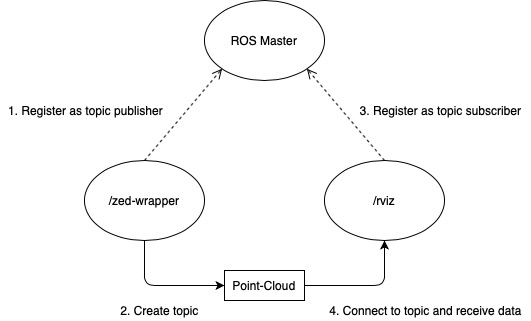
\includegraphics[width=0.8\linewidth]{img/ros_master_registration}
	\caption{Diagram of the topic registration process in ROS at which the publishing node registers its topic before the subscriber tells the master its interest in the point-cloud topic. However a node can be registered as a subscriber to a specific topic without the topic existing yet.}
		\label{fig:ros_master_reg}
\end{figure}



\section{Transform Library}
A complex robotic system consists of multiple parts such as sensors, cameras, manipulators, etc. which are each represented as a coordinate frame, where each frame is connected to another frame using joints. When trying to move a specific part or coordinate frame, not only the transform of that single frame but the composite transform of each frame in relation to the target has to be calculated. This is especially important when moving a robotic arm based on sensor readings. In this example a transform between the position of the sensor and the arm needs to be calculated so the motion performed by the arm the motion perceived by the sensor match.
Using the ROS Transform Library (tf) these complex calculations can be facilitated. To this end tf keeps track of each coordinate frame in a acyclic relationship tree where tf broadcasters then publish relative pose information and listeners query transforms between two coordinate frames. 
Because not all pose information in a robotic system is instantly accessible, the tf saves this information for each frame over time. This means that transforms can be queried not just spacially but also temporally.



\section{Simulation}
Debugging and testing robot applications can be a repetitive and tedious task, especially when a test environment needs to be reset at every test cycle. In order to facilitate this part of development the Autumn robot utilises the representation and simulation technologies that are described in the following sections.

\subsection{URDF}
In order to perform simulations or compute coordinate frame transforms a robot needs to be described in some way. One of the more popular description formats is the Unified Robot Description Format (URDF) which provides a XML format for representing a robot and its components as well as a \textit{C++} parser and tools to convert and verify and visualize these models. \footcite{openSourceRoboticsFoundationURDFNodate}
The \textit{check\_urdf} tool parses a URDF-File and returns the robots kinematic chain if successful.
To visualize the robots frames and joints in a graphviz\footcite{graphvizAuthorsAboutNodate} tree the \textit{urdf\_to\_graphiz} tool can be used. The resulting tree corresponds to the relationship tree tf uses to calculate transforms.

\subsection{Gazebo Simulator}\label{section:gazebo}
Gazebo is a 3D physics simulator often used in close relation to ROS projects. Therefore it provides tooling for model and world design and generation as well as comprehensive interfaces for controlling a simulated robot through ROS. Further advantages of Gazebo are its accurate sensor and sensor noise generation as well as its large community providing countless models of robots and sensors. \footcite{openSourceRoboticsFoundationGazeboNodate}
%vielleicht noch über URDF SDF schreiben - aber erst wenn simulation von autumn fertig ist

\filbreak
	
	\chapter{Methodology}

\textbf{Author: } 

\filbreak

	\chapter{Implementation}

\textbf{Author: } 

\filbreak
	\chapter{Experiment 1}

\textbf{Author: } 

\filbreak
	\chapter{Lessons learned}

\textbf{Author: } 

\filbreak
	\chapter{Experiment 2}

\textbf{Author: } 


\filbreak
	\chapter{Conclusion}

\textbf{Author: Fabian Kleinrad} 

\section{Autumn Result}

\subsection{Goal}
The objective of the autumn project is developing a fully autonomous drone capable of generating 3D scans of inaccessible areas. Additionally, it is possible to deploy the drone in regions lacking external localization based on the technologies used. Technologies realizing these features are already available. In contrast to these commercially available solutions, the autumn project aims to accomplish these feats using a low budget approach. 

\subsection{Design choices}
Crucial to the whole operation are means to perceive objects surrounding the drone. To accomplish this, a stereo camera was chosen due the to low cost compared to sensors used for commercial autonomous solutions.\newline
The drone used in the autumn project provides for a wide range of possible sensor configurations and a high payload capacity. This simplified prototyping and helped with the fast iterative approach used in this project. Using a smaller drone would have impeded tests due to the increased complexity of working with compact physical space and smaller weight margins.\newline
To enable computation on the drone itself, an NVIDIA-Jetson TX2 is being employed. This solves the issue of latency problems, which are especially troublesome in processes that need to perform without interruption to guarantee the most optimal results. In the case of the autumn project, such a process would be the continuous mapping of the environment.
\pagebreak
\subsection{Result}
The autumn drone performs mapping using stereo images provided by the stereo camera mounted on the drone. An RRT*-based path-planning algorithm then uses these mapping results to calculate a path originating from the drone's position to an selected end-point. The current position is also provided by the SLAM algorithm in the mapping stage. Using this route information, the drone can be controlled accordingly.
In the current version of the drone, only semi-autonomous flight is supported.Furthermore, due to the lack of testing possibilities and the risk that accompanies testing autonomous drones, flight capabilities were only assessed using user input.

\subsection{Mapping}
With the focus of autumn centring around creating 3D scans of environments, the aspect of mapping is a crucial factor upon which the quality of results depends on.\newline
Mapping was realized by implementing a 3D graph-based SLAM algorithm, supporting stereo imagery. The algorithm determines the current position of the device that provides the images. SLAM generates a point cloud representing the environment the drone explores based on this relative position. All mapping logic is computed on the drone using an NVIDIA-Jetson TX2, which provides enough computational power to ensure the most optimal results. In order to transfer the point cloud data, an access point is being hosted, over which a client may supervise the result. This enables the user to get a real-time view of the model and how it is being constructed. The resulting point-cloud can then be used as reference material in numerous applications.\newline
An example of its utilization would be the basis of a detailed render. In this scenario, it would simplify the process of measuring and conveying the composition into modelling software. The defining structure is already present using a point cloud, and only a few adjustments have to be made.

\subsection{Path-Planning}
Autonomy implies the means to navigate through an environment without external help. In autumn, this is realized using a path-planning algorithm. This algorithm is based on the RRT* algorithm, often employed in high-dimensional and dynamic domains. The algorithm plans a path through either a two-dimensional or three-dimensional representation of the environment surrounding the drone. In autumn, this model is being generated in the mapping phase using the SLAM algorithm.\newline
The path is computed separately from the drone. The reason is that separating the path computation onto an external device allows the drone to work more efficiently and the path-planning algorithm not to be constricted by computational restriction present when computing on the drone itself.\newline
The route is calculated between the drone's current position and a user-defined end-point. If newer mapping data is available, the previously generated path gets checked for possible collisions with newly scanned obstacles. Due to the single-query approach of the RRT algorithm, a new path has to be calculated in the case of the path being invalid.
The resulting path can be visualized for the user alongside the model generated in the mapping phase. This allows for early error detection through a human observer.

\section{Outlook}

\subsection{Current problems}
At current times, fully autonomous flight is not possible with the autumn drone. A significant risk factor in the design is the inability to monitor the space above the drone. This results in problems when using three-dimensional path-planning due to the uncertainty of what lies above. Without that information, the drone is unable to utilize the third dimension, which is the most crucial factor for using a UAV. In autumn, this was solved by focusing on a semi-autonomous approach.  
Another problem is the short battery life-time of the drone, which is due to the size of the drone used in the project. This leads to complications when scanning medium to large environments.  

\subsection{Future solutions}
The modular structure provided by ROS allows the autumn project to be easily implemented using different hardware. It is possible to realize fully autonomous flight using a smaller drone and a simpler two-dimensional lidar for future projects. This results in the loss of three-dimensional mapping capabilities but enables a more reliable and easier environment exploration.\newline 
Furthermore, using ROS, every part of the autumn logic can be used in separate projects where needed.
An example would be using the two-dimensional path-planning algorithm to plan the movement of a ground vehicle. 

\filbreak
	
	
	% Index
	\newpage
	\chapter*{Index}
	\printindex[name]
	\printindex[title]
	
	\printbibliography
	
	\chapter*{Messbox zur Druckkontrolle}



\begin{center}
{\Large --- Druckgröße kontrollieren! ---}

\bigskip

\Messbox{100}{50} % Angabe der Breite/Hoehe in mm

\bigskip

{\Large --- Diese Seite nach dem Druck entfernen! ---}

\end{center}



\end{document}
